%  LaTeX support: latex@mdpi.com
%  In case you need support, please attach all files that are necessary for compiling as well as the log file, and specify the details of your LaTeX setup (which operating system and LaTeX version / tools you are using).

% You need to save the "mdpi.cls" and "mdpi.bst" files into the same folder as this template file.

%=================================================================
\documentclass[buildings,article,submit,moreauthors,pdftex,10pt,a4paper]{mdpi} 

%--------------------
% Class Options:
%--------------------
% journal
%----------
% Choose between the following MDPI journals:
% actuators, admsci, aerospace, agriculture, agronomy, algorithms, animals, antibiotics, antibodies, antioxidants, applsci, arts, atmosphere, atoms, axioms, batteries, behavsci, beverages, bioengineering, biology, biomedicines, biomimetics, biomolecules, biosensors, brainsci, buildings, carbon, cancers, catalysts, cells, challenges, chemosensors, children, chromatography, climate, coatings, computation, computers, condensedmatter, cosmetics, cryptography, crystals, data, dentistry, designs, diagnostics, diseases, diversity, econometrics, economies, education, electronics, energies, entropy, environments, epigenomes, fermentation, fibers, fishes, fluids, foods, forests, futureinternet, galaxies, games, gels, genealogy, genes, geosciences, geriatrics, healthcare, horticulturae, humanities, hydrology, informatics, information, infrastructures, inorganics, insects, instruments, ijerph, ijfs, ijms, ijgi, inventions, jcdd, jcm, jdb, jfb, jfmk, jimaging, jof, jintelligence, jlpea, jmse, jpm, jrfm, jsan, land, languages, laws, life, literature, lubricants, machines, magnetochemistry, marinedrugs, materials, mathematics, mca, mti, medsci, medicines, membranes, metabolites, metals, microarrays, micromachines, microorganisms, minerals, molbank, molecules, mps, nanomaterials, ncrna, neonatalscreening, nutrients, particles, pathogens, pharmaceuticals, pharmaceutics, pharmacy, philosophies, photonics, plants, polymers, processes, proteomes, publications, recycling, religions, remotesensing, resources, risks, robotics, safety, sensors, separations, sexes, sinusitis, socsci, societies, soils, sports, standards, sustainability, symmetry, systems, technologies, toxics, toxins, universe, urbansci, vaccines, vetsci, viruses, water
%---------
% article
%---------
% The default type of manuscript is article, but can be replaced by: 
% addendum, article, book, bookreview, briefreport, casereport, changes, comment, commentary, communication, conceptpaper, correction, conferencereport, expressionofconcern, meetingreport, creative, datadescriptor, discussion, editorial, essay, erratum, hypothesis, interestingimage, letter, newbookreceived, opinion, obituary, projectreport, reply, retraction, review, sciprints, shortnote, supfile, technicalnote
% supfile = supplementary materials
%----------
% submit
%----------
% The class option "submit" will be changed to "accept" by the Editorial Office when the paper is accepted. This will only make changes to the frontpage (e.g. the logo of the journal will get visible), the headings, and the copyright information. Also, line numbering will be removed. Journal info and pagination for accepted papers will also be assigned by the Editorial Office.
%------------------
% moreauthors
%------------------
% If there is only one author the class option oneauthor should be used. Otherwise use the class option moreauthors.
%---------
% pdftex
%---------
% The option pdftex is for use with pdfLaTeX. If eps figure are used, remove the option pdftex and use LaTeX and dvi2pdf.

%=================================================================
\firstpage{1} 
\makeatletter 
\setcounter{page}{\@firstpage} 
\makeatother 
\articlenumber{x}
\doinum{10.3390/------}
\pubvolume{xx}
\pubyear{2016}
\copyrightyear{2016}
\externaleditor{Academic Editor: name}
\history{Received: date; Accepted: date; Published: date}
%------------------------------------------------------------------
% The following line should be uncommented if the LaTeX file is uploaded to arXiv.org
%\pdfoutput=1

%=================================================================
% Add packages and commands here. The following packages are loaded in our class file: fontenc, calc, indentfirst, fancyhdr, graphicx, lastpage, ifthen, lineno, float, amsmath, setspace, enumitem, mathpazo, booktabs, titlesec, etoolbox, amsthm, hyphenat, natbib, hyperref, footmisc, geometry, caption, url, mdframed
\usepackage{textcomp}

%=================================================================
%% Please use the following mathematics environments:
 \theoremstyle{mdpi}
 \newcounter{thm}
 \setcounter{thm}{0}
 \newcounter{ex}
 \setcounter{ex}{0}
 \newcounter{re}
 \setcounter{re}{0}

 \newtheorem{Theorem}[thm]{Theorem}
 \newtheorem{Lemma}[thm]{Lemma}
 \newtheorem{Corollary}[thm]{Corollary}
 \newtheorem{Proposition}[thm]{Proposition}

 \theoremstyle{mdpidefinition}
 \newtheorem{Characterization}[thm]{Characterization}
 \newtheorem{Property}[thm]{Property}
 \newtheorem{Problem}[thm]{Problem}
 \newtheorem{Example}[ex]{Example}
 \newtheorem{ExamplesandDefinitions}[ex]{Examples and Definitions}
 \newtheorem{Remark}[re]{Remark}
 \newtheorem{Definition}[thm]{Definition}
%% For proofs, please use the proof environment (the amsthm package is loaded by the MDPI class).

%=================================================================
% Full title of the paper (Capitalized)
\Title{Impact of Heat Pumps Flexibility in a French Residential Eco-District}

% Authors, for the paper (add full first names)
\Author{Camille Pajot $^{1}$*, Benoit Delinchant $^{1}$, Yves Maréchal $^{1}$ and Damien Frésier $^{2}$}
% Authors, for metadata in PDF
\AuthorNames{Camille Pajot, Benoit Delinchant, Yves Maréchal and Damien Frésier}

% Affiliations / Addresses (Add [1] after \address if there is only one affiliation.)
\address{%
$^{1}$ \quad Univ. Grenoble Alpes, CNRS, Grenoble INP, G2Elab, 38000 Grenoble, France; benoit.delinchant@g2elab.grenoble-inp.fr, yves.marechal@g2elab.grenoble-inp.fr\\
$^{2}$ \quad Gaz et Electricité de Grenoble, 57 Rue Pierre Semard, 38000, Grenoble, France; d.fresier@geg.fr}

% Contact information of the corresponding author
\corres{Correspondence: camille.pajot1@g2elab.grenoble-inp.fr; Tel.: +3-347-682-7080}

% Simple summary
%\simplesumm{}

% Abstract (Do not use inserted blank lines, i.e. \\) 
\abstract{This paper investigates how blocks of buildings could fit into load shedding strategies. It deals in particular with the effects on peak shaving, occupants’ thermal comfort or CO$_{2}$  emissions reduction and how to quickly quantify them.
To achieve this goal, the paper focuses on a new residential district, thermally fed by heat pumps. Four modeling approaches were confronted in order to estimate buildings' responses to load shedding orders. 
At the district scale, it may be necessary to mix modeling approaches, from experimental results to detailed thermal models. Accuracy is not guaranteed for all approaches so that the choice should be made carefully in regards to study needs. However, results are sufficient to conclude on the load shedding effects.
By cutting hourly heating load, building by building, the strategy has proved itself efficient for both peak shaving and thermal comfort. With a very diffuse rebound effect, most of the heating load cut during the peak period is shifted during low-consumption periods providing an effective peak shaving, while the thermal comfort is guaranteed at least 96\% of the time. For CO$_{2}$ emissions reduction, the link between consumption reduction and CO$_{2}$ emissions savings should be realized carefully, since shifting the consumption could increase these emissions.
}

% Keywords
\keyword{Peak Shaving; Demand Response; Block of Buildings; Thermal Model; TEASER}

% The fields PACS, MSC, and JEL may be left empty or commented out if not applicable
%\PACS{J0101}
%\MSC{}
%\JEL{}

% If this is an expanded version of a conference paper, please cite it here: enter the full citation of your conference paper, and add $^\S$ in the end of the title of this article.
%\conference{}

%%%%%%%%%%%%%%%%%%%%%%%%%%%%%%%%%%%%%%%%%%
% Only for the journal Data:

%\dataset{DOI number or link to the deposited data set in cases where the data set is published or set to be published separately. If the data set is submitted and will be published as a supplement to this paper in the journal Data, this field will be filled by the editors of the journal. In this case, please make sure to submit the data set as a supplement when entering your manuscript into our manuscript editorial system.}

%\datasetlicense{license under which the data set is made available (CC0, CC-BY, CC-BY-SA, CC-BY-NC, etc.)}

%%%%%%%%%%%%%%%%%%%%%%%%%%%%%%%%%%%%%%%%%%
\begin{document}

%%%%%%%%%%%%%%%%%%%%%%%%%%%%%%%%%%%%%%%%%%
%% Sections that are not mandatory are listed as such. The section titles given are for Articles. Review papers and other article types have a more flexible structure. 

\section{Introduction}
% % % % % % % % % % % % % % % % % % % % % % % % % % % % % %
\subsection{Background}
Nearly 3 years after the 21$^{th}$ Conference of the Parties of the UNFCCC (COP21), lots of energy transition policies have been carried out in order to respect Paris Agreement by keeping the global average temperature  below 2\textdegree{}C above pre-industrial levels \cite{noauthor_paris_nodate}.
The massive integration of renewable energy sources, together with the electrical peak consumption augmentation put load flexibility in a central position into energy transition strategies, as it could help to guarantee grid stability \cite{lund_review_2015}.

Lots of new stakeholders, as well as new markets, appear in order to modulate electrical consumption \cite{ponds_aggregator_2018}. However, aggregators mostly apply these demand response strategies on electricity-intensive industries, excluding lower power level sites such as buildings. % ref 
Nevertheless, the latter represent a large share of energy consumption, so that they can represent a significant amount of power if gathered. Thanks to their thermal inertia, they also appear as a great candidate for short punctual or repeated heat load shedding orders, but this flexibility remains hard to quickly evaluate.

Therefore it became one of the key points studied in the European project City-zen \cite{noauthor_city-zen_nodate}. Our work together with the local DSO (Distribution System Operator) GEG (Grenoble Electricity and Gas) takes place in this context and focus on a new residential eco-district. This district (23 buildings for 264 flats) is thermally fed by ground source heat pumps (GSHP), placing the heating as an electrical issue. Indeed, GSHP represent a significant research field \cite{congedo_cfd_2012, congedo_computational_2014}, so that they are at the cutting edges of research with the demand side management (DSM) in order to manage electric grid constraints \cite{razmara_building--grid_2017}.

\subsection{Context and aims of the study}
Into the local context of Grenoble, an electrical morning consumption peak appears between 5 am and 10 am so that GEG is interested in peak shaving by giving efficient load shedding orders.  However, it could be hard to quickly quantify the impact of load shedding strategies on peak shaving, but also to avoid any occupants' thermal discomfort as well as any carbon footprint increase.

Indeed, the problem can be complex to model. On the one hand, in order to maintain the occupants' thermal comfort, some load shedding can be realized after an over-heating so that the building could store heat before stopping the heating systems. On the other hand, as it induces an over-consumption, this over-heating should be performed before the peak period (in our case between 5 am and 10 am), when the purpose is to reduce the consumption peak. In order to study a strategy of district peak reduction by stopping the heating supply building by building, two load shedding strategies (with or without over-heating) will be compared. 

This paper aims to quickly quantify the influence of this district heat load shedding strategy on the heat load curve, the thermal comfort and greenhouse gases emissions reduction. Moreover, the study will try to quantify the impact of the heat load profiles modeling on the results.


\subsection{Literature review}	% Previous work
On the one hand, peak-shaving strategies are widely studied in order to deal with electric grid constraints \cite{UDDIN20183323}. On the other hand, DSM becomes more studied at a local scale \cite{MULLER2015283}, focusing on local energy integration \cite{salpakari_improved_2016}, demand curve smoothing \cite{zhang_linearized_2018} or economic purposes \cite{behrangrad_review_2015}. These two combined lead to an increase of research papers on the field of peak-shaving for a better management of local electric grid constraints through DSM \cite{Baeten_2017}.

The idea of using buildings' thermal inertia in order to modulate the heating load becomes more and more studied in the literature too. While buildings' flexibility is studied will several aims such as increasing district heating systems efficiency \cite{kensby_potential_2015,romanchenko_thermal_2018} or for a better integration of local production sources \cite{reynders_potential_2013}, it is also investigated with the objective to evaluate what could be their future impact in smartgrids \cite{de_coninck_bottom-up_2013} and to compare them to storage solutions \cite{le_dreau_energy_2016}. Several methodologies have been developed in order to quantify this flexibility but only three are commonly applied using building structural mass \cite{reynders_energy_2018}. Moreover, only a few of these papers evaluate the impact on thermal comfort as they mostly consider it as a constraint \cite{reynders_generic_2017}. In our case, the possibility to be out of the comfort zones will be considered, usually defined by set-point temperature ranges \cite{aduda_demand_2016,le_dreau_energy_2016}, while estimated this impact by standing on comfort ranges defined in \cite{faria_neto_thermal_2016}.

Most of the time, estimating the building temperature is possible as the building thermal flexibility quantification is based on thermal models. These models can be from low-order RC model \cite{goy_estimating_2017} to higher-detailed models often based on widespread tools such as EnergyPlus \cite{le_dreau_energy_2016, hurtado_quantifying_2017} or based on the Modelica language such as the library IDEAS \cite{reynders_quality_2014}. 
Even the district scale becomes more and more widespread into the energetic dynamic simulation software, as DIMOSIM (DIstrict MOdeller and SIMulator) developed by the CSTB \cite{perez_contribution_2017}, CEA (City Energy Analyst) from the Zurich ETH \cite{fonseca_city_2016} or TEASER (Tool for Energy Analysis and Simulation for Efficient Retrofit) from RWTH \cite{remmen_teaser:_2018}.
However, it was shown that this scale change could be dangerous by being relevant for annual heating needs, but not anymore when focusing on power analysis \cite{frayssinet_adaptation_2017}. For this reason, models with different levels of details have been studied.

\subsection{Paper structure}	% Previous work
In the present paper, the first section details the methods used for the load shedding impact quantification. At first, the impact indicators in terms of peak shaving, thermal comfort and CO$_2$ reduction will be defined. Then, the heat load profiles modeling will be presented. Finally, the load shedding scenarios studied in the paper will be introduced. In the 'Results' section, the two load shedding strategies will be analyzed on a building thanks to the indicators previously introduced. The results will show the impact on the three aspects: peak-shaving, thermal comfort, and CO$_2$ emissions while analyzing the effect of the heat load profiles modeling. Finally, the paper will end with conclusions based on the observed results.

%%%%	MethodS		%%%%
\section{Methods for load shedding impact quantification}

\subsection{Load shedding impact quantification indicators}

\subsubsection{Peak shaving}
In order to quantify at best the amount of load reduction in a district, the key indicators will be defined first. Many studies show some rebound effects after a load shedding, related to the restart of the consumption \cite{morales_assessment_2017}. This behavior could not only affect the energy conservation by providing any (or few) consumption reductions at a daily scale, but it could also lead to a failure for the peak shaving strategy. Indeed, if concentrated during a short period, a load shifting could cause bigger grid constraints during this time period.
For this reason, in order to quantify the impacts of load shedding strategies for peak shaving purposes, the behavior of the consumption report after the end of the load shedding period has to be analyzed. To do so, the study is based on one indicator used by the French TSO RTE \cite{RTE_rapport_report}. The daily Load Shifting rate (LS$_{rate}^{d})$) is defined in equation \ref{daily_LS_eq} from the ratio of the addition of anticipated energy and delayed energy, by the cut-off energy. These three energies are defined in equations \ref{cut_off_eq} to \ref{delayed_eq} by the integral in a given period of the consumption power (P$_{t}$) and its reference value without operation (P$^{ref}_{t})$. These energies are also visible in Fig. \ref{multiple-load-shedding}.

\begin{equation}
    \label{daily_LS_eq}
    LS_{rate}^{d} = \frac{E_{anticipated} + E_{delayed}}{E_{cut\_off}}
\end{equation}

Where :
\begin{equation}
\label{cut_off_eq}
E_{cut\_off} = \int_{\tau_{ls}^b}^{\tau_{ls}^e} P_{t}^{ref}\, \mathrm{d}t
\end{equation}

\begin{equation}
\label{anticipated_eq}
    E_{anticipated} = \int_{\tau_{ls}^{b} - 1}^{\tau_{ls}^{b}} (P_{t} - P_{t}^{ref})\, \mathrm{d}t   
\end{equation}

\begin{equation}
\label{delayed_eq}
    E_{delayed} = \int_{\tau_{ls}^{e}}^{\tau_{ls}^{e} + 23} (P_{t} - P_{t}^{ref})\, \mathrm{d}t
\end{equation}

By taking into account the energy reported during the 23 hours following the load shedding, this indicator gives information at a daily scale. However, in order to get a better understanding of the dynamic behavior of this energy report, the study will rather focus on an adapted form of this load shifting rate, defined in equation \ref{LS_dyn_rate}. This indicator will be calculated hourly in order to quantify the distribution of energy report, hour by hour, as shown in figure \ref{load_shed_repres}.

\begin{equation}
\label{LS_dyn_rate}
LS_{rate}^{h} = \frac{ \int_{h}^{h+1}(P_{t} - P_{t}^{ref})\, \mathrm{d}t}{E_{cut\_off}}
\end{equation}

\begin{figure}[H]
    \centering
    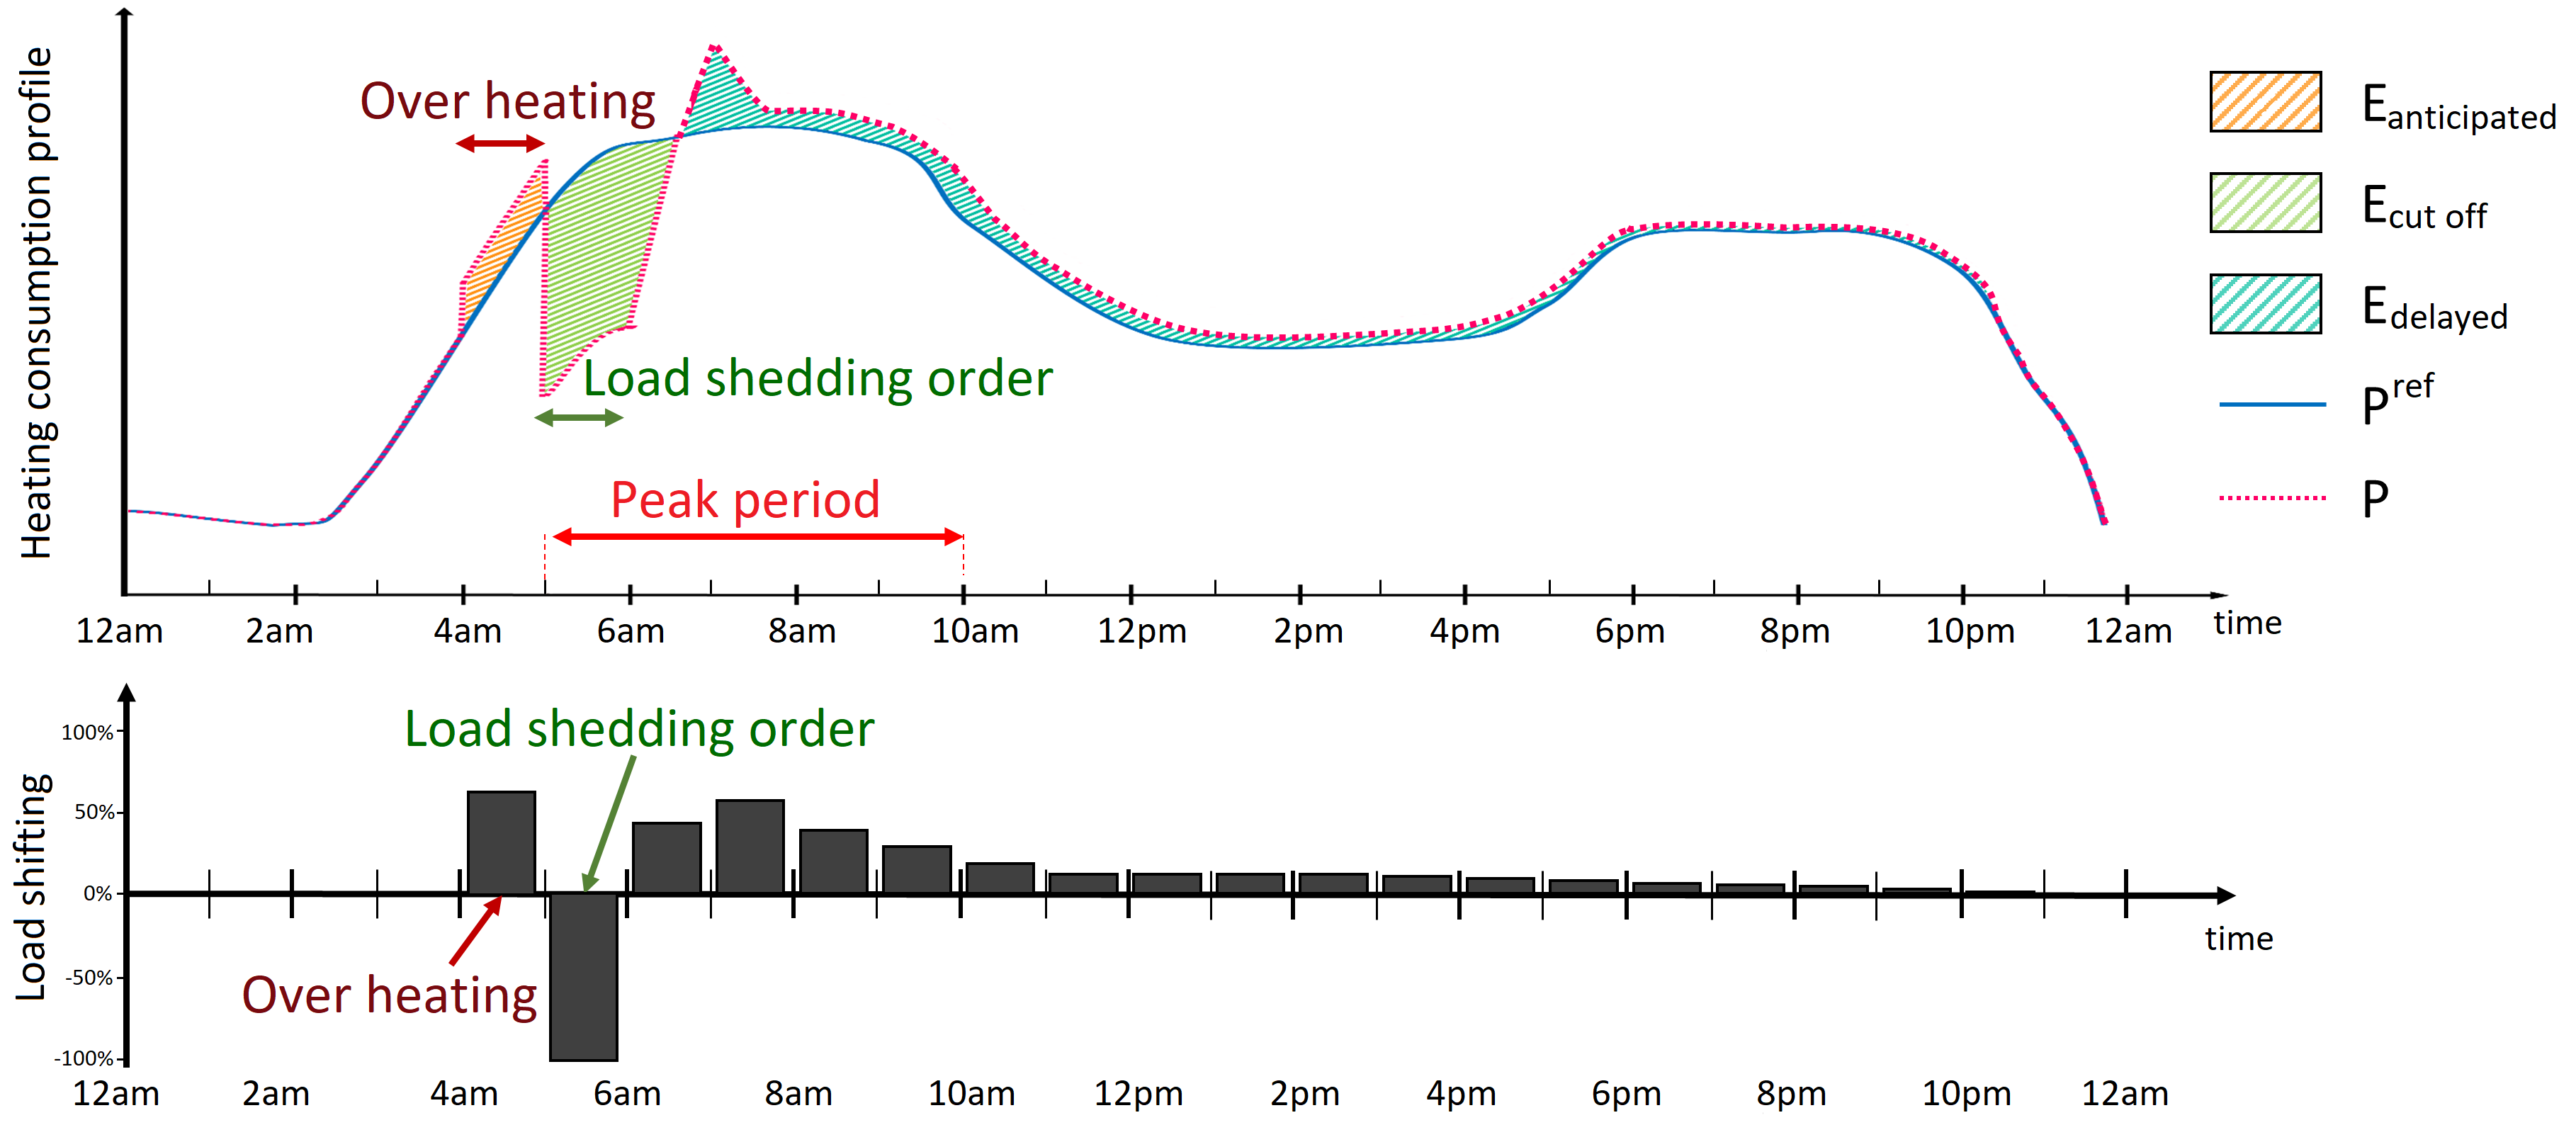
\includegraphics[scale=0.2]{Effacement_et_taux_de_report_en.png}
    \caption{Representation of a daily heating load curve modification with a load shedding order and associated load shifting rates.}
    \label{load_shed_repres}
\end{figure}

Defined as such, the load shifting rate can be used to study dynamically the load variations and gives information on the efficiency of the load shedding strategy to reduce a long peak period (more than one hour).

\subsubsection{Thermal comfort}
It is important to keep in mind that stopping the heat supply can impact the thermal comfort so that this aspect has to be estimated too. When cutting the heating supply of a building, the internal temperature does not decrease instantaneously to the level of external temperature. This building dynamic can be explained by the possibility for buildings to store heat into their heavy components, such as walls. Indeed, due to their important inertia, walls will cool lower than the air, in cases of heating load shedding. The phenomena are important in terms of comfort, as walls and air temperatures respectively reflect radiation and convection effects perceived by the occupants of the building. Since the feeling of thermal comfort is related to this perception of both air and walls temperature, studies analyzed the relationship between thermal comfort and the operative temperature (T$_{op}$, defined eq. \ref{eq_Top}) \cite{de_dear_developing_1998}.

\begin{equation}
	\label{eq_Top}
	T_{op} = \frac{T_{walls} + T_{air}}{2}
\end{equation}

In this study, this operative temperature will be taken as indicator in order to estimate the comfort level, according to levels defined in \cite{faria_neto_thermal_2016}:

\begin{itemize}[leftmargin=*,labelsep=4mm]
	\item Comfortable: A range of +/- 1\textdegree{}C about the temperature set-point (T$_{set}$)
	\item Slightly uncomfortable: A range of +/- 1\textdegree{}C and +/- 2\textdegree{}C about T$_{set}$
	\item Uncomfortable: A difference of more than 2\textdegree{}C with T$_{set}$
\end{itemize}

\begin{figure}[H]
    \centering
    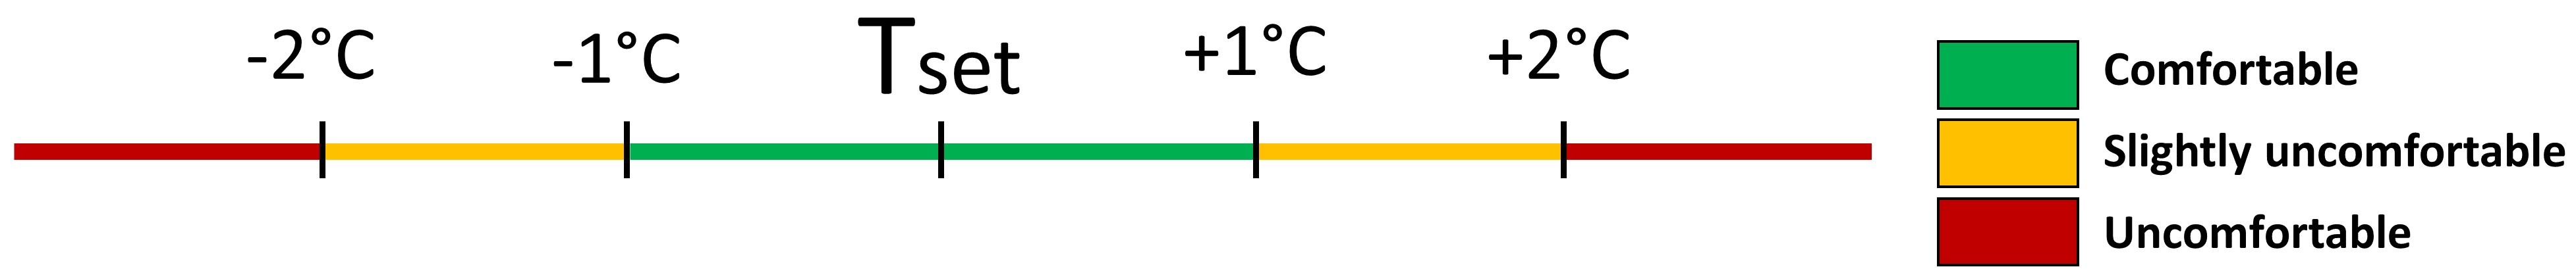
\includegraphics[scale=0.4]{Temperature_comfort.jpg}
    \caption{Comfort levels associated to the difference between T$_{op}$ and T$_{set}$}
    \label{temp_comfort}
\end{figure}

\subsubsection{CO$_{2}$ emissions reduction}
% Entire section to rephrase
Finally, the impact of the different load shedding methods on CO$_{2}$ emissions will be studied. To do so, the work will rely on the actual CO$_{2}$ emissions from the French power generation during January 2016 \cite{noauthor_eco2mix_2014}. 
This will allow us to estimate the gross CO$_{2}$ emissions variation when the load shedding strategies will be applied while taking into account hourly and daily variation (see equation \ref{co2_red_eq}). 

\begin{equation}
\label{co2_red_eq}
    CO_{2}S^{m} = \frac{\int_{month}(CO_{{2}_{t}}^{ref} - CO_{{2}_{t}})\, \mathrm{d}t}
    {\int_{month}(CO_{{2}_{t}}^{ref})\, \mathrm{d}t }
\end{equation}

However, this variation does not only take into account the load shifting, but also the consumption reduction. Moreover, it is very common to conclude that CO$_2$ emissions will obviously decrease with load shedding strategies when there are some energy savings. A widespread indicator for these energy savings is the daily Energy Saving rate (ES$_{rate}^{d}$) defined as follows :

\begin{equation}
    ES_{rate}^{d} = \frac{E_{cut\_off} - E_{anticipated} - E_{delayed}}{E_{cut\_off}}
\end{equation}

This energy saving rate is commonly used to quantify energy sobriety in the long-run by showing the amount of non-reported energy 23 hours after \cite{RTE_rapport_report}. Nevertheless, the energy savings rate should be put in perspective, as it only represents savings in regard to cut-off energy. Therefore the energy savings on an entire day is much lower than ES$_{rate}^{d}$, so that with this logic daily CO$_2$ emissions reduction would be lowered too.

\begin{equation}
\label{ES_month}
    ES^{m} = \frac{\int_{month}(P_{t}^{ref} - P_{t})\, \mathrm{d}t}{\int_{month}(P_{t}^{ref})\, \mathrm{d}t}
\end{equation}

Nevertheless, this does not prevent us to expect that CO$_2$ emissions would decrease as much as daily consumption. To examine deeper the impact on district carbon footprint, it is crucial to consider the daily and intra-day CO$_2$ emission variability for the electrical production system. Thus, moving electrical consumption from a time period to another one could increase the CO$_2$ emissions, when local peaks don't match to global electrical system ones.

For all these reasons, the paper will compare the total consumption reduction (ES$^{m}$) to the total CO$_{2}$ emissions reduction during the month (CO$_2$S$^{m}$). The comparison will gather the two reductions (energy consumption and CO$_2$ emissions) into a single indicator the Expected Gain reduction (EG$_{red}$), defined as follows :

\begin{equation}
    EG_{red} = \frac{ES^{m} - CO_{2}S^{m}}{ES^{m}}
\end{equation}


%% HEAT LOAD PROFILES MODELS %%
\subsection{Heat load profiles models}
According to the indicators previously defined, at least the heat load variation between no-load shedding orders and the applied load shedding strategy need to be assessed in order to quantify the impact on peak shaving and CO$_2$ emissions. In the present study, two modeling types will be compared. At first, a standard load shifting profile will be established with experimental data. Then, thermal models with several levels of details will be introduced in order to assess thermal comfort. 

% Experimentation
\subsubsection{Experimental load shifting profile}
A first estimation can rely on experimental results from similar buildings and load shedding strategies. The main advantage of this method is to assess very quickly the peak shaving indicator.
To do so, a standard load shifting rate profile was defined, based on experimental results from the French GreenLys project \cite{noauthor_annuaire_nodate} 
and from a study led by the French TSO RTE \cite{RTE_rapport_report}.
As the experimental building stock contains two new eco-districts \cite{noauthor_annuaire_nodate}, the use of the resulting standard profile is considered suitable for our new residential district. The experimental results show an energy saving rate around 90\% and the load shifting rate profiles are plotted below.

\begin{figure}[H]
	\centering
   	\begin{minipage}[c]{7.5cm}
      	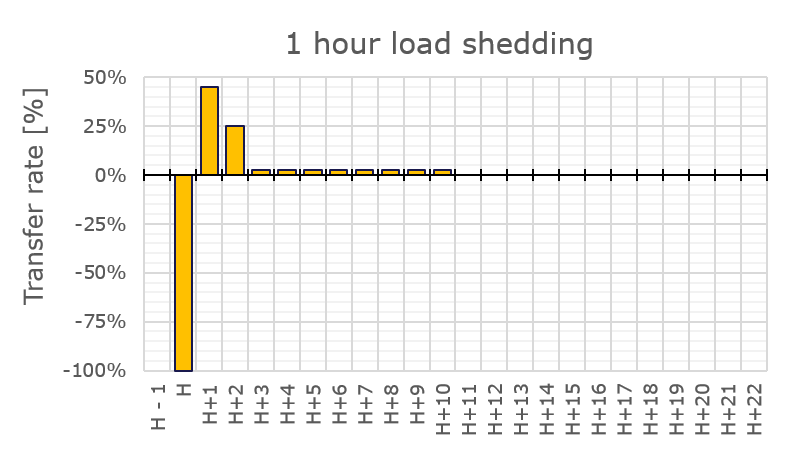
\includegraphics[width=7.5cm, trim=30 0 0 33, clip=true]{Figure_1.png}
   \end{minipage} \hfill
   \begin{minipage}[c]{7.5cm}
        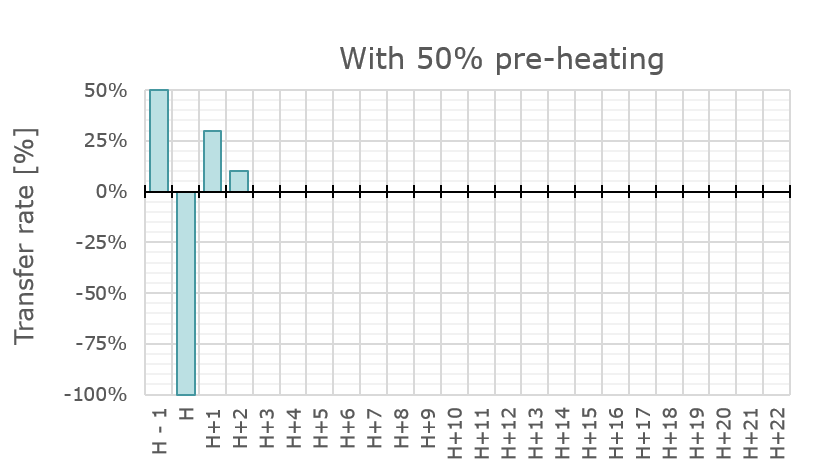
\includegraphics[width=7.5cm, trim=20 0 0 36, clip=true]{Figure_2.png}
   \end{minipage}
 
   \caption{Load shifting rate profiles.(\textbf{a}) One-hour residential heat load shedding without pre-heating (\textbf{b}) One-hour residential heat load shedding after one-hour pre-heating}
   \label{exp_lt_profile}
   
\end{figure}

On the left side figure \ref{exp_lt_profile}(\textbf{a}) is represented the hourly load shifting rates for a one-hour residential heat load shedding without pre-heating, while figure \ref{exp_lt_profile}(\textbf{b}) shows it after an over-heating of one hour, consuming 50\% of the cut-off energy.

% Thermal models
\subsubsection{Thermal models}
\label{thermal_models}
In order to quantify the impact on thermal comfort, it is also necessary to estimate T$_{op}$ (cf. equation \ref{eq_Top}). For this reason, two thermal models with identified parameters were used in order to simulate the building dynamic during and after the load shedding. 

In order to manage both modelings (thermal model of the building and electric model of the grid), while being an open-source tool, TEASER \cite{fuchs_workflow_2016} was chosen for the first thermal model creation. It allows to automatically generate RC thermal models in the Modelica language for the AixLib \cite{noauthor_aixlib:_2018} and the Annex60 \cite{noauthor_modelica-ibpsa:_2018} libraries.

The thermal model can be created thanks to building envelope information (wall areas, orientations, thickness, materials, ...). However, as it can be very difficult at the district scale to access to the specific data about each building envelope, this can also be realized with at least 5 inputs data: year of construction, net area, type of use, number of floors and height of floors \cite{fuchs_workflow_2016}, making the tool very useful to save time. If only these data are given, the tool will enrich the dataset thanks to statistical data, whose use in a French context will be analyzed in this study case.

\begin{figure}[H]
	\centering
    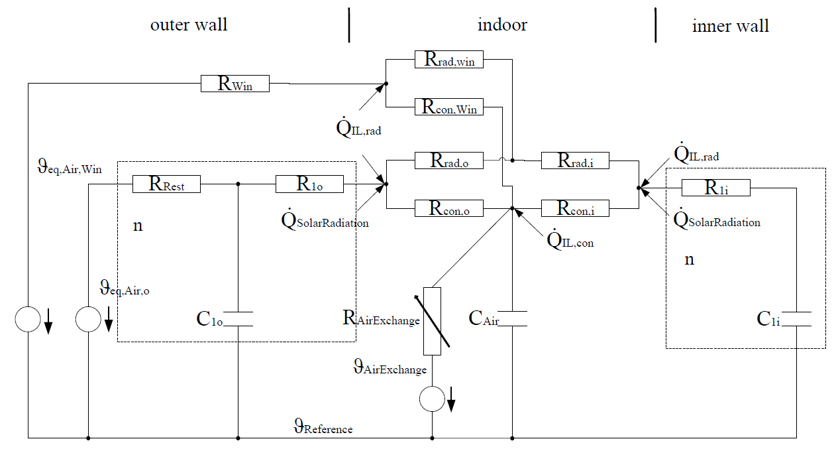
\includegraphics[width=10cm]{RC_model.png}
    \caption{Scheme of the RC equivalent model generated by TEASER}
    \label{RC_model_TEASER}
\end{figure}

Therefore, for the same thermal model structure (see figure \ref{RC_model_TEASER}), two precision levels can be achieved depending on the input data. In order to compare the impact of dataset enrichment, both the model generated with the 5 minimal parameters and the model enriched with the building envelope data were analyzed. The first one will further be referred as the 'Simple' model, while the second one enriched with data used for the regulatory Building Energy Simulation (BES) will further be referred as the 'Enriched' model.

%%% Second model %%%
The second one is the fully detailed thermal model used for the mandatory study. Indeed, in a French context, since each building construction requires an energetic study based on a fully detailed thermal model, existing thermal models from this mandatory study can also be re-used.
In this study, a Pleiades tool \cite{pleiades} has been used to build a detailed model (each room is considered as a thermal zone), that will be called 'Complex' model afterward.

For all heat load profiles from simulation models, the result from a thermal dynamic simulation of a building in our district was considered as reference heat load profile (P$_{t}^{ref}$). The building behavior in case of a temperature set-point of 20\textdegree{}C was simulated during the month of January. All other data: weather, occupancy schedules, internal gains for lightning etc. have been set to the same values in order to get a better comparison between simulation results.
However, the set-point temperatures for the 'Simple' and 'Enriched' models are ambient temperatures, while the one in 'Complex' model is on the operative temperature, and cannot be changed. Therefore, small differences between the results could still be expected.

\subsubsection{Modeling approaches summary}
To summarize, four modeling approaches are considered in order to estimate the load shifting rates is this paper:
\begin{itemize}[leftmargin=*,labelsep=4mm]
	\item The 'Standard' model: the statistical model from experimental data
	\item The 'Simple' model: thermal model generated by TEASER (fig.\ref{RC_model_TEASER}) with database
	\item The 'Enriched' model: thermal model generated by TEASER (fig.\ref{RC_model_TEASER}) with building envelope data
	\item The 'Complex' model: multi-zone thermal model created with a Pleiades tool
\end{itemize}

%%% Load shedding scenarios %%%
\subsection{Load shedding scenarios modeling}

For these models, two scenarios will be studied :
\begin{itemize}[leftmargin=*,labelsep=4mm]
	\item One-hour heat load shedding after one-hour over-heating: In order to over-heat the building out of the peak period (5 am to 10 am), the load shedding order will be applied from 5 am to 6 am.
	\item Simple one-hour heat load shedding: In this scenario, the load shedding order will be applied in the middle of the peak period, from 7 am to 8 am without any over-heating.
\end{itemize}

Each load shedding will be obtained by a very low set-point temperature (around 0\textdegree{}C) in order to cut the heat supply. The aim of these two scenarios is to represent the two load shedding types that could be made building by building into the district. For instance, by applying the first strategy (with over-heating) to a first building and then applying the second strategy to each of four other building hour by hour, the resulting load shedding on the entire district would be obtained by adding the individual effects (see figure \ref{multiple-load-shedding}). 

\begin{figure}[H]
\centering
	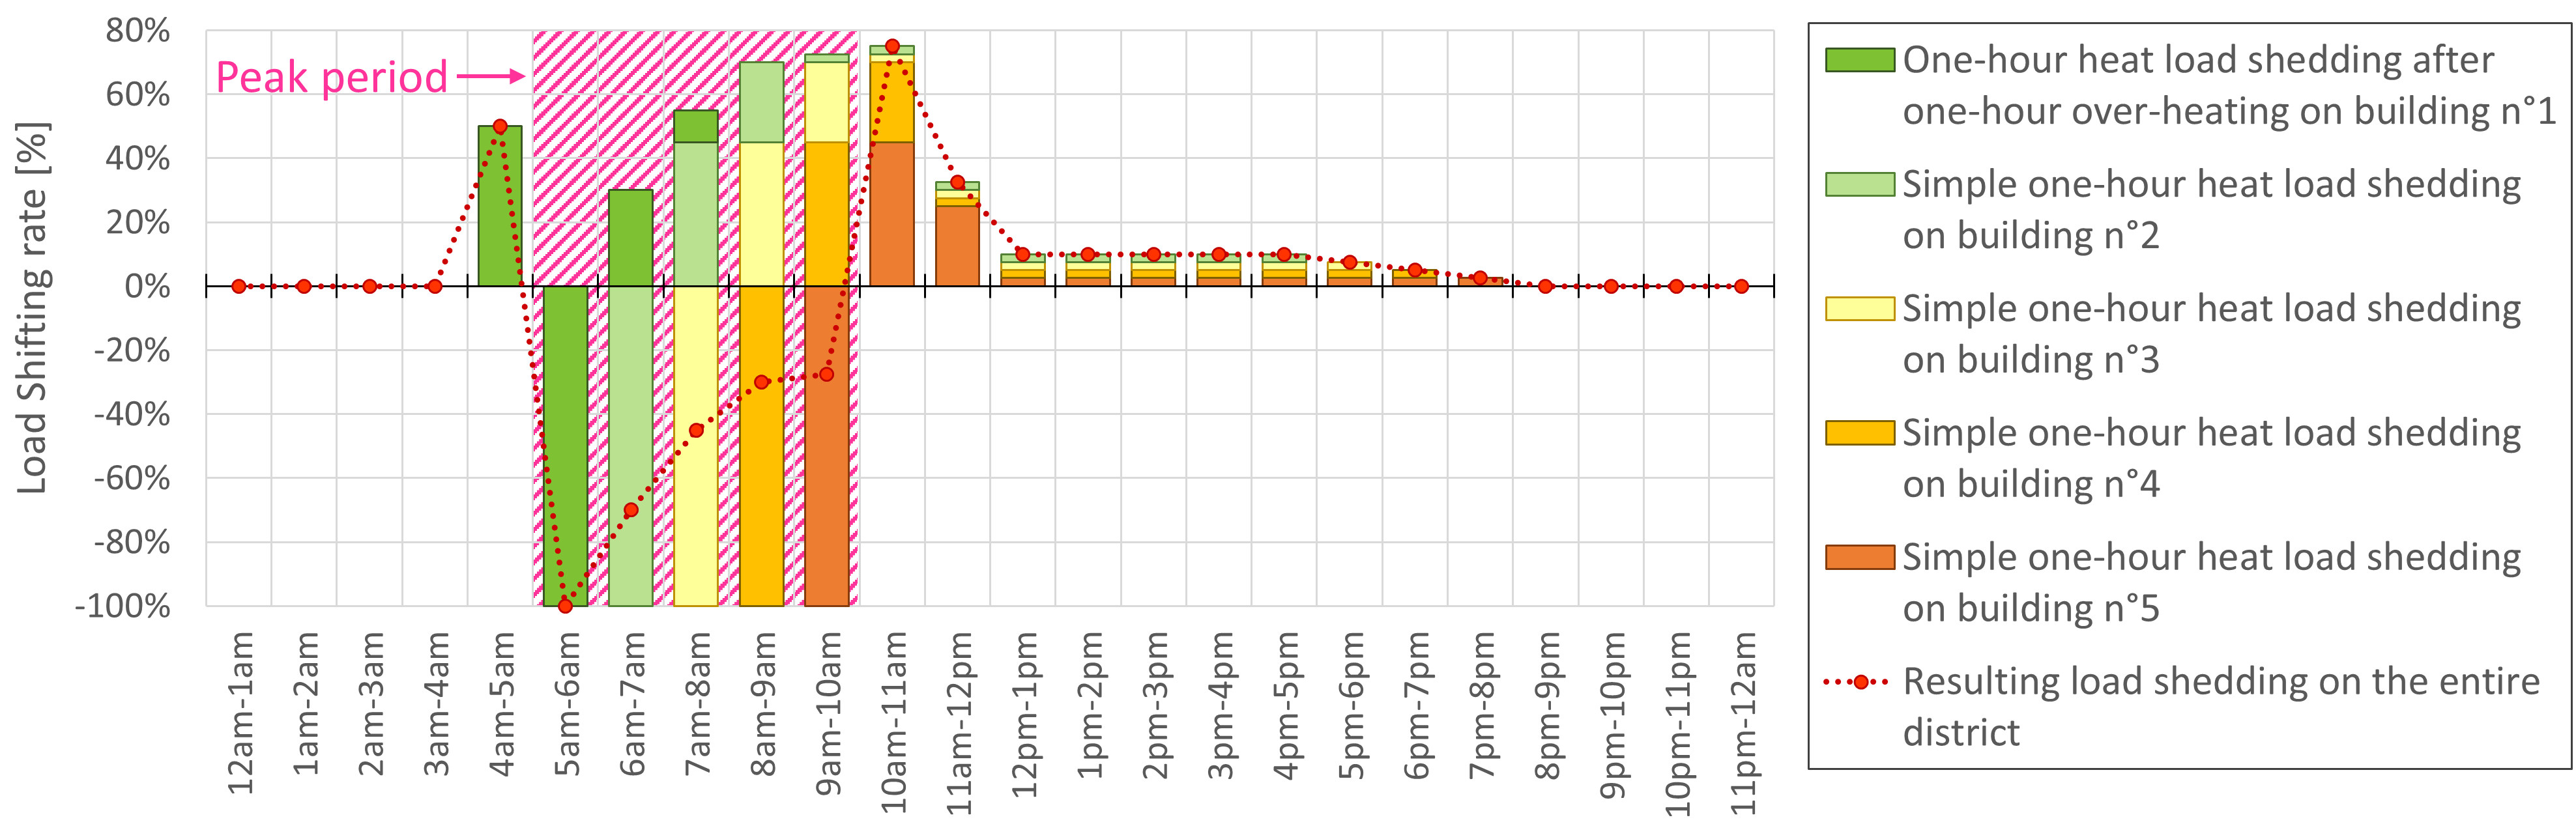
\includegraphics[width=15cm]{Figure_3.png}
	\caption{Load shifting rate profiles during a day for the multiple one-hour heat load shedding from 5 am to 10 am. Example of the 'Standard' model for load shifting rate profiles for 5 buildings.}
    \label{multiple-load-shedding}
\end{figure}


%%%%%%%%%%%%%%%%%%%%%%%%%%%%%%%%%%%%%%%%%%
\section{Results and discussion}
The load shedding impacts in terms of peak shaving, thermal comfort and CO$_2$ emissions will be analyzed in this section. 
As explained previously, the district load-shedding strategy consists in cutting heating load building by building during one-hour. The first load shedding would integrate a one-hour over-heating the previous hour, while all the following orders will be simple one-hour heat load shedding. Two different building behaviors are thus expected for these two strategies.

%% RESULTS - Peak Shaving %%
\subsection{Results for peak shaving}
\label{results_peak_shaving}
%%%%%%%%%%%%%%%%%%%%%%%%%%%%%%%%%%%%%%%%%%%%%%%%%%
%%%% Not sure it is useful to separate the strategies in results %%%

In order to reduce the mean power during the peak period, the load shifting rate would have to be the more diffuse as possible to shift most of the consumption out of the peak period. Thus, the lower load shifting rates, the more the load shedding would be considered as efficient for peak shaving. As two dynamic responses are expected from the building depending on whether it has been previously over-heated or not, results will be exposed for the two load shedding strategy. At first, results for a simple heat load shedding happening from 7 am to 8 am each day of the month of January will be drawn. Then, the second load shedding strategy with a one-hour over-heating before cutting the heat supply will be shown. This load shedding will be applied from 5 am to 6 am, in order to shift the anticipated consumption before the peak period.

\subsubsection{Heat load shedding from 7 am to 8 am}
In figure \ref{simple-load-shedding-res}, are displayed the results of the simple one-hour load shedding applied all days of January. The mean load shifting can be found for all of the four modeling approaches ('Standard', 'Simple', 'Enriched' and 'Complex'). The mean operative temperatures are also drawn with their variation range during the month. 
\begin{figure}[H]
	\centering
	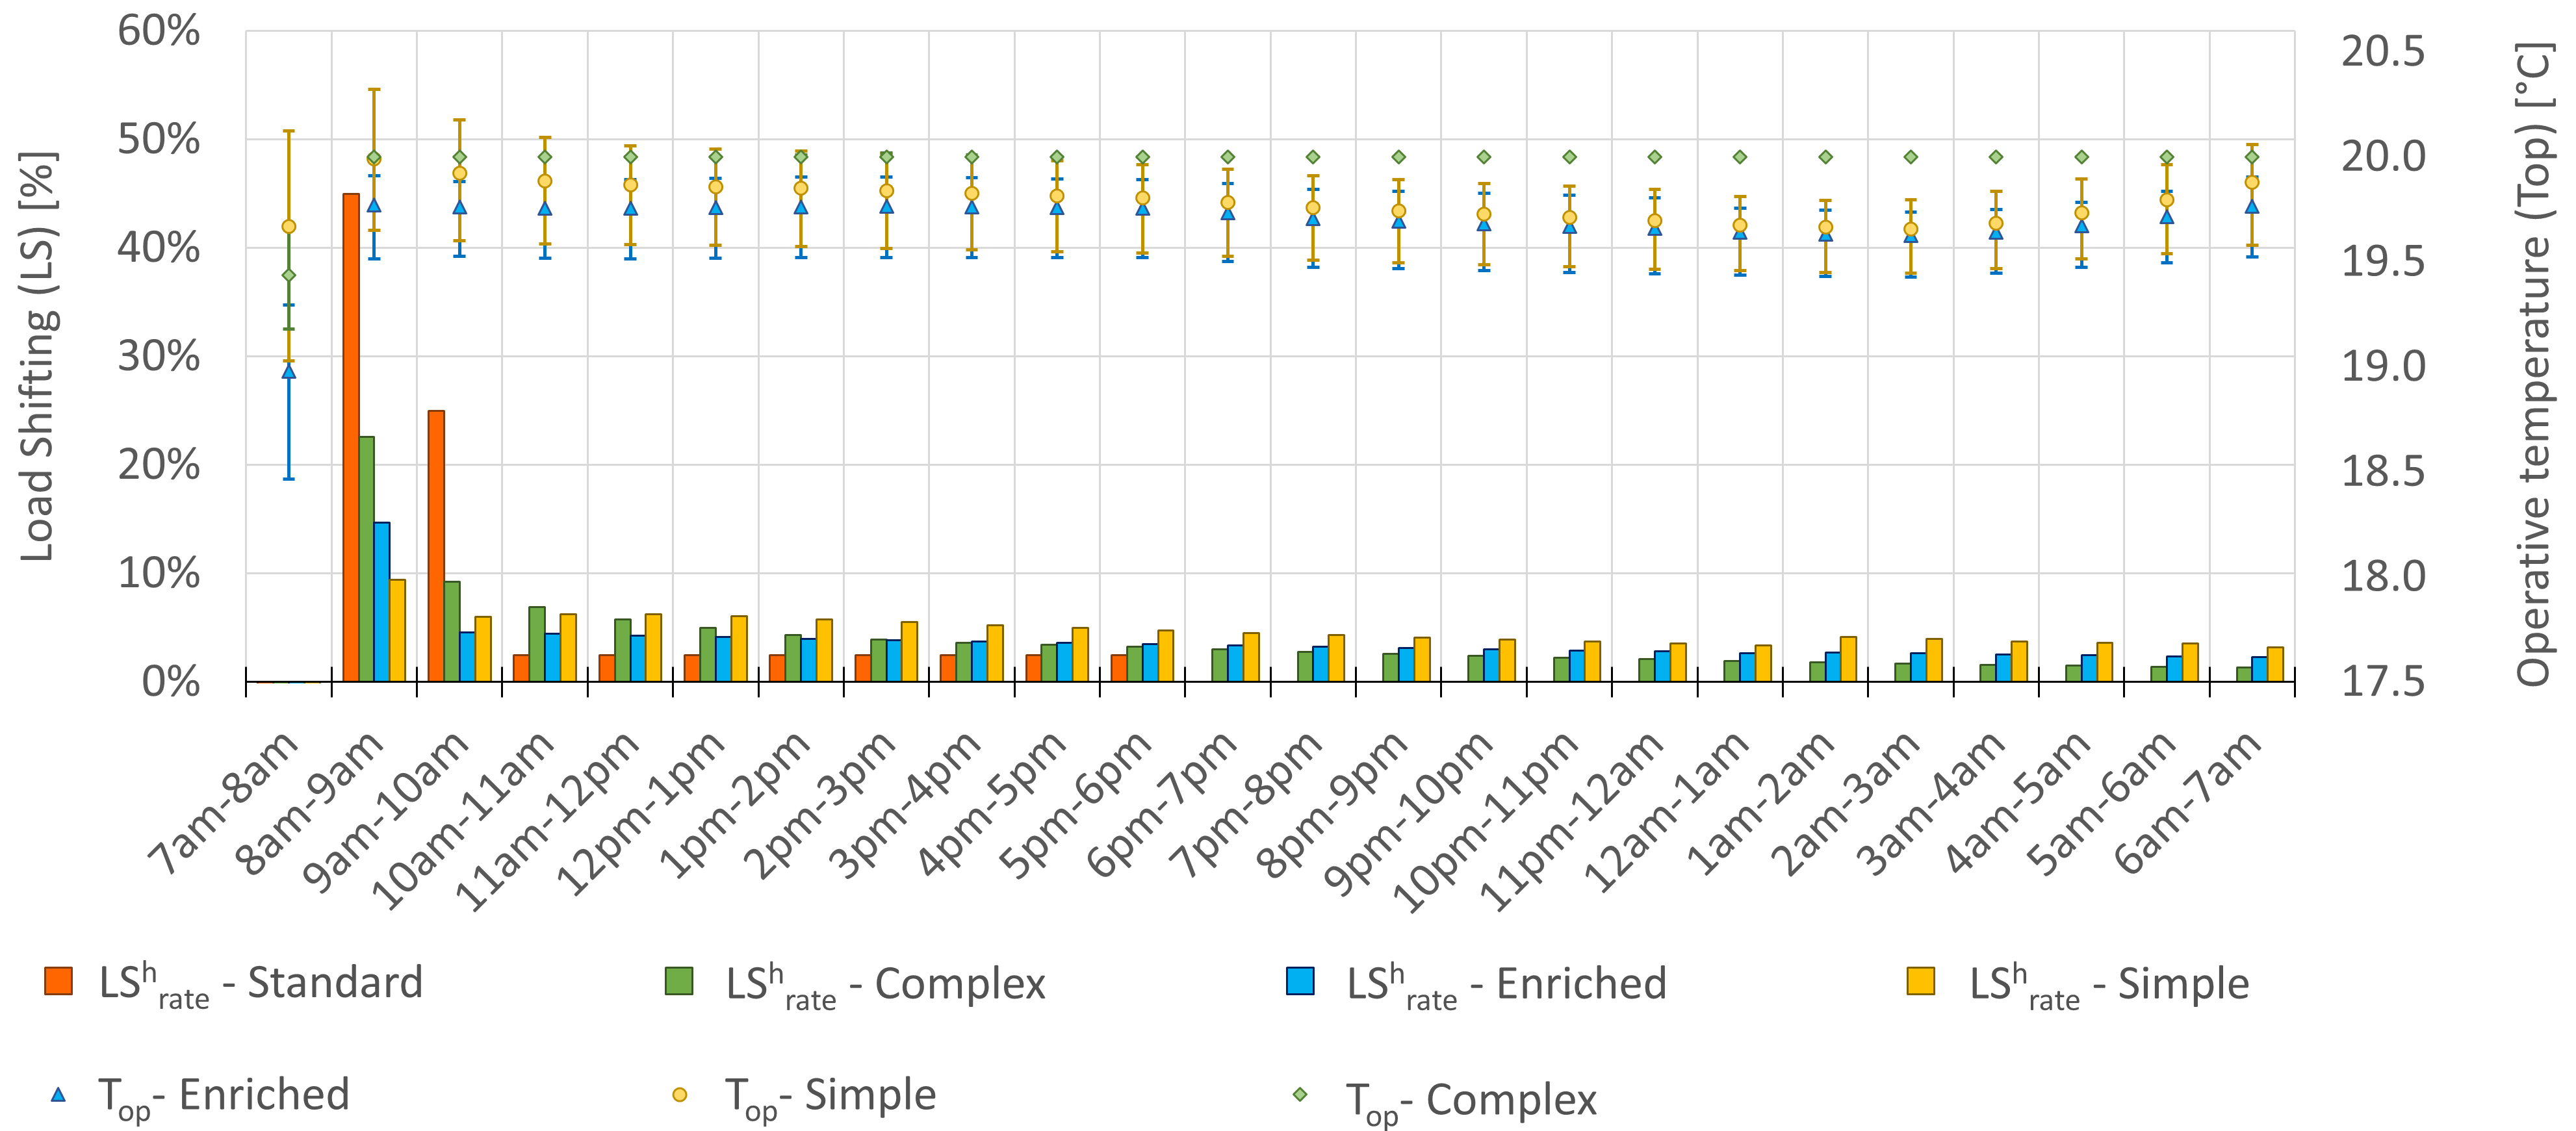
\includegraphics[width=15cm]{simple_ls.png}
  	\caption{One-hour heat load shedding}
    \label{simple-load-shedding-res}
\end{figure}
      
Two main different building behaviors can be observed for this strategy:
\begin{itemize}[leftmargin=*,labelsep=4mm]
	\item Most of the rebound effect appears within the two hours following the load shedding (experimental load shifting profile)
	\item The cut consumption is shifted during the entire day (load shifting profiles from thermal models)
\end{itemize}

Here, it can be noticed that all the simulation results from thermal models show a slower dynamic than the experimental load shifting profile.

\subsubsection{Heat load shedding from 5 am to 6 am after an over-heating from 4 am to 5 am}
In figure \ref{complex-load-shedding-res} are presented the results of the complex one-hour heat load shedding strategy, taking place from 5 am to 6 am after a one-hour over-heating. The strategy was applied each day of January and results are the average value for each time slot and each modeling, like those presented in figure \ref{simple-load-shedding-res}. As seen before, there is a big difference between experimental and simulated buildings behaviors for simple heat load shedding strategy. This gap between models is therefore confirmed for this complex strategy too.

\begin{figure}[H]
	\centering
	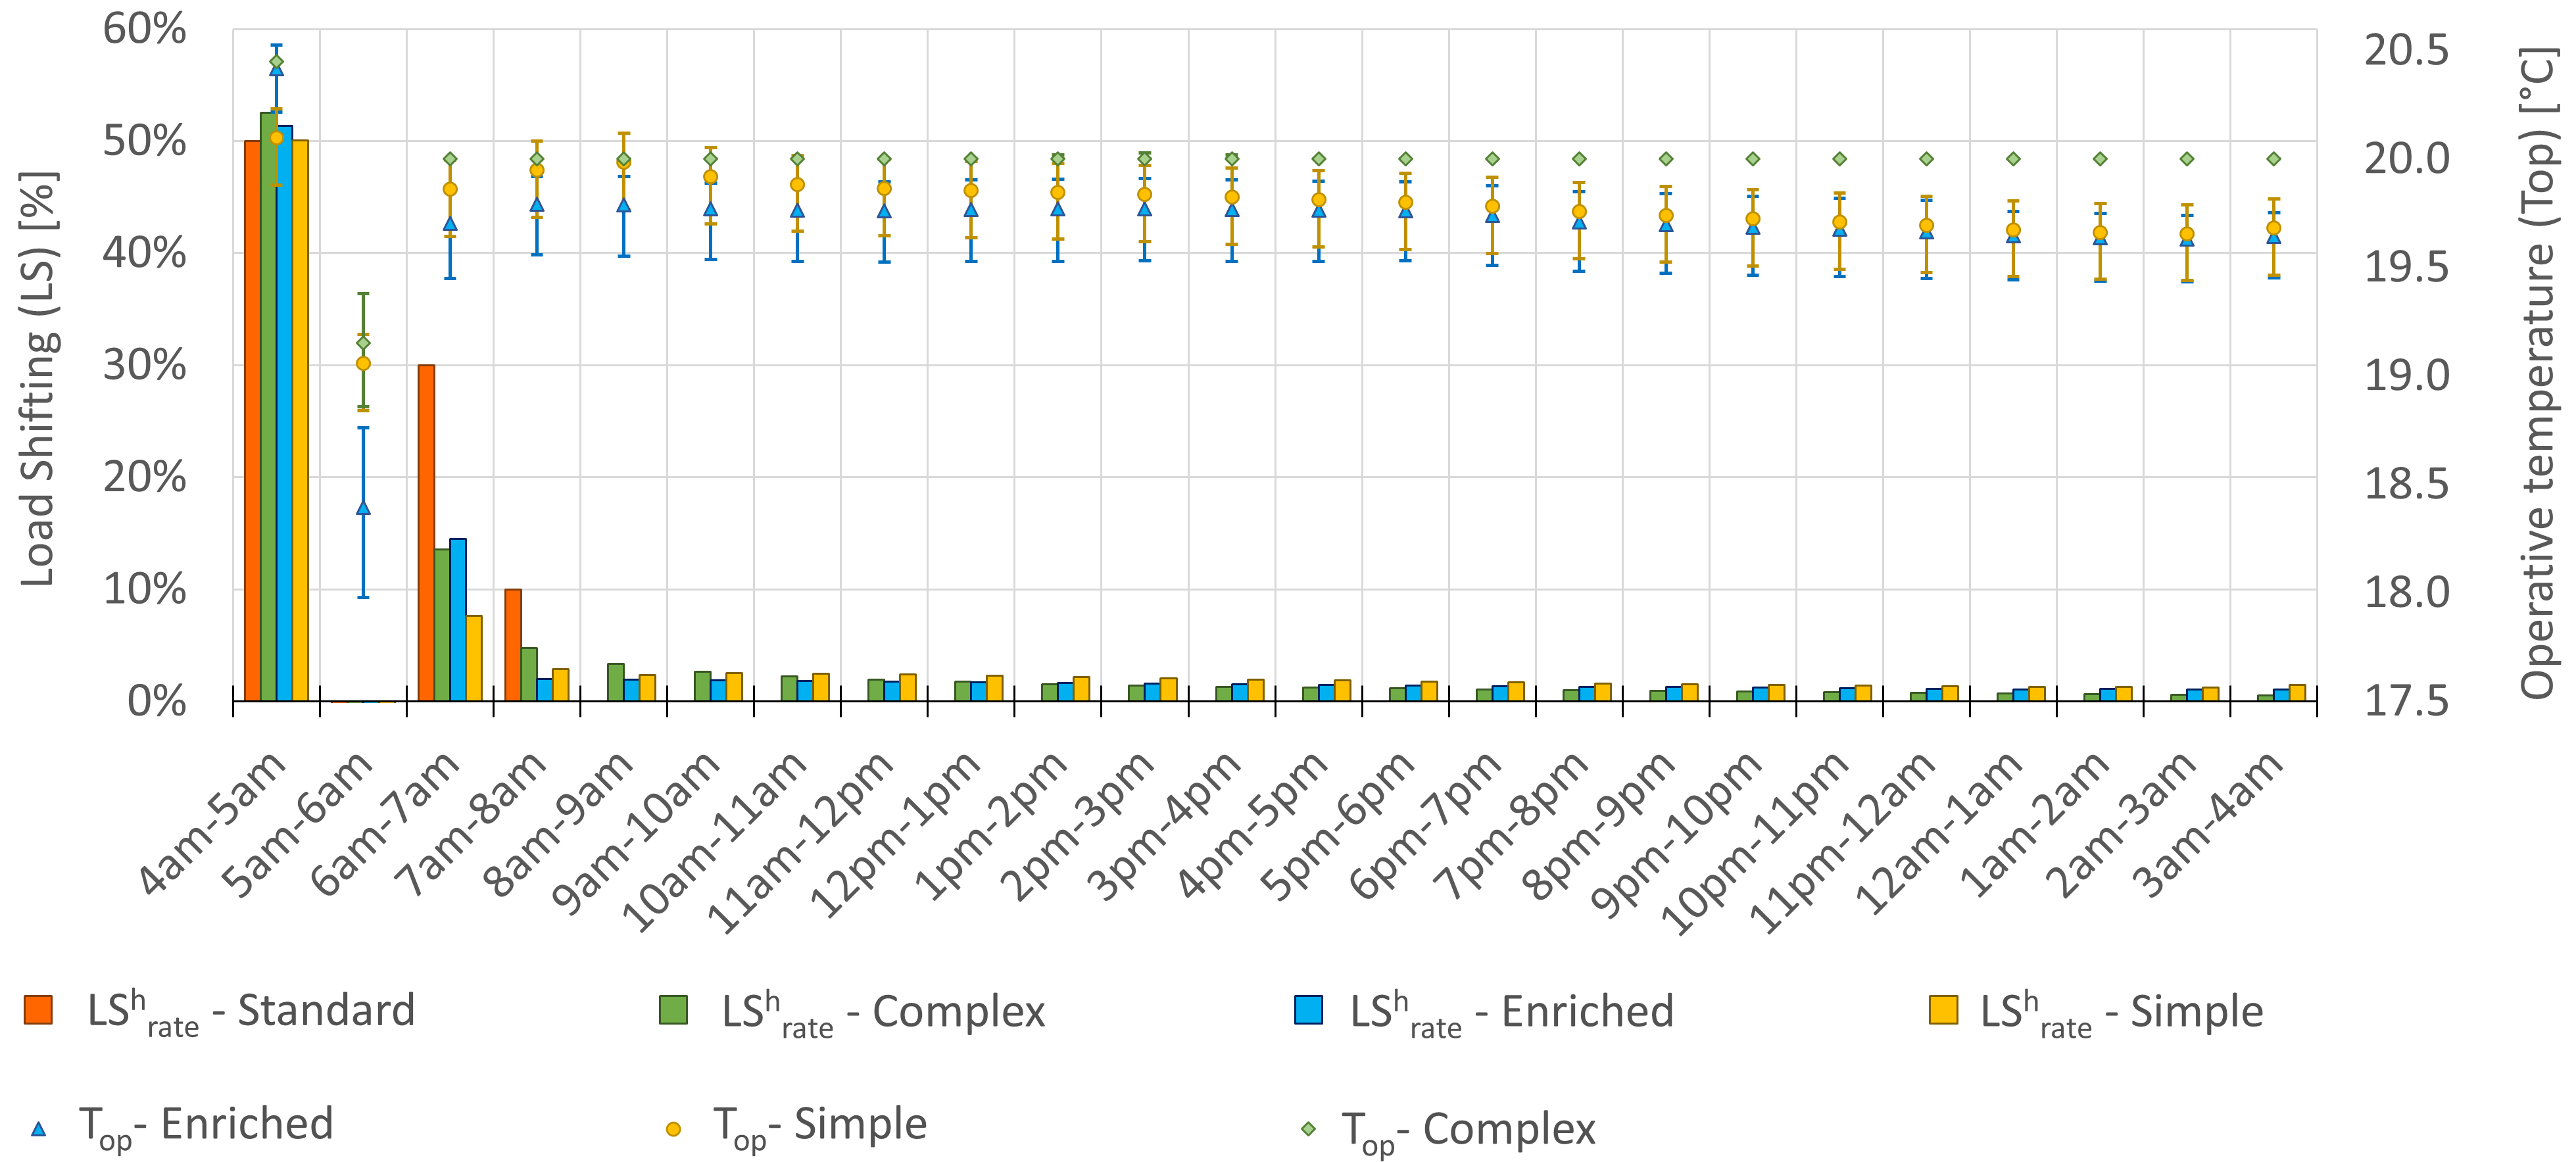
\includegraphics[width=15cm]{pre_heating_ls.png}
	\caption{One-hour heat load shedding after one-hour over-heating}
    \label{complex-load-shedding-res}
\end{figure}

Although this standard profile was established from real measurement, it remains difficult to consider it as more reliable than simulated profiles. Indeed, weather and occupancy data differ and several types of buildings are aggregated. Even with less old buildings than new ones in the experiment, consumption values for heating tend to be higher for the first category and mean values could be strongly affected. In spite of this conclusion, the standard model reminds that occupancy behavior could play a great role in the rebound effect. In our study case, the heating load is entirely controlled by the building manager, so that this effect can be neglected.

Thus, conclusions on the effect of the global strategy (starting with the complex strategy and going on, building by building, with the simple load shedding) could be realized by analyzing the building behaviors predicted by thermal models. These three modeling approaches all lead to diffuse energy reports so that it can be concluded that this load shedding strategy could be efficient in regard to a peak shaving objective, even if thermal comfort still need to be looked at.

%% RESULTS - Thermal comfort %%
\subsection{Results for thermal comfort}
As explained before, the study focuses on the building operative temperature as thermal comfort indicator. With a set-point temperature fixed to 20\textdegree{}C, the comfort zone is reached over 19\textdegree{}C and below 21\textdegree{}C. Results obtained for the month of January are presented in figures
\ref{simple-load-shedding-res}  and \ref{complex-load-shedding-res}.
Mean operative temperatures are represented, with their variation intervals, so that it can be noticed that :
\begin{itemize}[leftmargin=*,labelsep=4mm]
	\item On average, load shedding hours are slightly uncomfortable
	\item On average, other hours of the days are comfortable
\end{itemize}

Distribution of comfort level for occupants for the load shedding strategy after an over-heating is presented in the tables below : 
% Results table
\begin{table}[H]
\centering
\caption{Thermal comfort levels distribution for the load shedding after over-heating strategy}
      \begin{tabular}{lccc}
      \hline
      & \multicolumn{3}{c}{Load shedding after over-heating} \\
      \hline
       Comfort level / Models & Reduced & Enriched & Complex \\
      Comfortable & 98.5\% & 96\% & 100\% \\
      Slightly uncomfortable & 1.5\% & 3.6\% & 0\% \\
     Uncomfortable & 0\% & 0.4\% & 0\% \\
     \hline
     \end{tabular}
\end{table}

Similar results are obtained for the load shedding strategy without over-heating. Most of the hours are "comfortable" (at least 96\% of the time for all models) and "uncomfortable" level is rarely reached (0.4\% of the time and only with the 'Enriched' model). However, further studies on the impact of heating systems (as shown in \cite{reynders_potential_2013}) or on the perception of this comfort could be needed to consolidate these results (as studied in \cite{amasuomo_perceived_2016}). As internal gains and external temperatures differ each hour, each time slot should be considered individually for further studies in the entire district impact. Finally, requiring less energy for heating purposes, new low-consumption buildings could get a large part of their heating needs from internal gains (lightning, devices, occupation, etc.). This would also have to be considered carefully in order to avoid an under-evaluation of thermal discomfort in buildings.

%\begin{table}[H]
%\centering
%\caption{Thermal comfort levels distribution for load shedding after over-heating strategy}
%      \begin{tabular}{lccc}
%      \hline
%      & \multicolumn{3}{c}{Load shedding after over-heating} \\
%      \hline
%      Comfort level / Models & Simple & Enriched & Complex \\
%      Comfortable & 98,5\% & 96\% & 100\% \\
%      Slightly uncomfortable & 1,5\% & 3,6\% & 0\% \\
%     Uncomfortable & 0\% & 0,4\% & 0\% \\
%     \hline
%     \end{tabular}
%\end{table}

%Paradoxically, more discomfort is generated in the case of the complex strategy including over-heating. This can be explained by the fact that the two strategies are not considered for the same time slot, so that internal gains and external temperatures are not the same. From this observation, it can be concluded that each time slot should be considered individually for further studies in the entire district impact.

%% RESULTS - CO2 emissions %%
\subsection{Results for CO$_2$ emissions reduction}
In this last section are presented the results for the impact on the carbon footprint. The chosen indicator for the effect is the expected gain reduction (EG$_{red}$), representing the difference between CO$_2$ emissions reduction expected by looking at the energy consumption savings (ES$^{m}$) and the effective CO$_2$ emission diminution (CO$_{2}$S$^{m}$). In order to put into perspective the feeling of savings obtained by looking at the mean ES$_{rate}^{d}$, the following table \ref{results_CO2} will also integrate it in comparison to the effective consumption reduction during the month (ES$^{m}$).

\begin{table}[H]
\caption{Consumption and CO$_2$ emissions reduction during January for the simple load shedding strategy (a) and for the load shedding after over-heating strategy (b)}
\label{results_CO2}

% Change names
    \begin{minipage}{0.5\textwidth}
        \centering
              \begin{tabular}{lccc}
              \hline
              & \multicolumn{3}{c}{Load shedding} \\
              \hline
               Models & Simple & Enriched & Complex \\
             ES$_{rate}^{d}$ & -10,0\% & 13,1\% & 5,5\%\\
             ES$^{m}$ & 0,40\% & 0,50\% & 0,22\% \\
             CO$_{2}$S$^{m}$ & 0,38\% & 0,50\% & 0,16\% \\
             EG$_{red}$ & 3,2\% & 0,70\% & 28\% \\
             \hline
             \end{tabular}
    \end{minipage}
    \begin{minipage}{0.5\textwidth}
        \centering
              \begin{tabular}{lccc}
              \hline
              & \multicolumn{3}{c}{Load shedding after over-heating} \\
              \hline
               Models & Simple & Enriched & Complex \\
             ES$_{rate}^{d}$ & 3,1\% & 2,1\% & 2,4\% \\
             ES$^{m}$ & 0,21\% & 0,22\% & 0,14\% \\
             CO$_{2}$S$^{m}$ & 0,01\% & 0,05\% & -0,06\% \\
             EG$_{red}$ & 94\% & 76\% & 144\% \\
             \hline
             \end{tabular}
    \end{minipage}
\end{table}

For the load shedding between 7 am and 8 am (simple load shedding), the intuition is confirmed since the overall consumption reduction leads to the reduction of the CO$_2$ emissions, though a little less as expected. However, for the second strategy with overheating, CO$_2$ emissions reduction is not so obvious anymore. Depending on the models, the expected CO$_2$ emissions reduction is lower than the calculated one. It goes from 76\% less than expected to an increase of 44\% of CO$_2$ emissions. The reason for these differences is that the load is transferred from a low-CO$_2$ emissions time slot to higher CO$_2$ emissions times of the day.
In order to be consistent with energy transition strategies, it is important to consider this aspect into load shedding impact evaluation to avoid a local amelioration to the detriment of general interest.

%% If the documentclass option "submit" is chosen, please insert a blank line before and after any math environment (equation and eqnarray environments). This ensures correct linenumbering. The blank line should be removed when the documentclass option is changed to "accept" because the text following an equation should not be a new paragraph. 

%%%%%%%%%%%%%%%%%%%%%%%%%%%%%%%%%%%%%%%%%%

\section{Conclusions}
% Models comparison
With often few data available at the district scale, thermal models with parameters from the statistical database could provide coherent load shedding impacts results, in respect to those available with detailed thermal simulation models. However, a comparison between simulation results and measurements would be necessary to validate the accuracy of the results, although it was unfortunately impossible due to a lack of data on the considered buildings and external factor as occupation schedules and weather data. For our study case, thermal models are considered as reliable for trend estimations on the effects on peak shaving, thermal comfort and CO$_{2}$ emissions reduction for a first approach at a district scale. The global strategy for the district studied in this paper relies on two load shedding approaches :
\begin{itemize}[leftmargin=*,labelsep=4mm]
    \item An overheating from 4 am to 5 am before load shedding from 5 am to 6 am
    \item One-hour load shedding building by building beginning from 6 am to 9 am
\end{itemize}
% Load shedding results
The two approaches were analyzed separately on the three aspects :
\begin{itemize}[leftmargin=*,labelsep=4mm]
    \item \textbf{Peak shaving}\\
    Cutting the heating load during one hour building by building in an entire district seems to be effective for peak-shaving. Indeed, the transferred load is very diffuse (LS$_{rate}^{h}$<25\% the first hour and LS$_{rate}^{h}$<10\% the following hours) so that the rebound effects of the previous buildings do not cancel the peak reduction obtained by the current load shedding. These results are crucial in the case of a long peak (more than an hour), offering the possibility to shift the load outside consumption peak period.\\
    \item \textbf{Thermal comfort}\\
    Thermal comfort can be reduced during the load-shedding hours. Measurements would have to be realized in order to determine if operative temperature evaluation is more reliable when based on the 'Simple' model, the 'Enriched' model or the 'Complex' model. Indeed, the 'Complex' model assessed only 0.8\% of the time as not comfortable, while this discomfort could cover up to 4\% of the time with the 'Enriched' model. The different modeling approaches used do not allow to estimate precisely how much thermal comfort can be reduced and how it will be perceived by occupants but help the stakeholder to know that it can be an issue. In all cases, one solution to investigate in order to reduce thermal discomfort could be to reduce heat loads instead of cutting them or cutting during shorter durations.\\
    \item \textbf{CO$_{2}$ emissions reduction}\\
    In the case of CO$_2$ emissions reduction, estimation cannot be based only on consumption reduction as CO$_2$ emissions for electrical systems have dynamic variations that have to be taken into account. Only by considering dynamic CO$_{2}$ variations and by calculating the difference between emissions with or without load shedding strategy could lead to a reliable estimation of CO$_{2}$ emissions variations. Indeed, even with effective consumption diminution, a load shedding strategy could shift consumption from low-CO$_{2}$ periods to higher-CO$_{2}$ time slots, increasing the global CO$_{2}$ emissions. For instance, in the case of the load shedding after over-heating, the 'Complex' model assessed 0.14\% of energy savings during the month, while the CO$_{2}$ emissions increased from 0.06\%. Therefore, links between energy savings and CO$_{2}$ emissions reduction have to be realized carefully.
\end{itemize}

Finally, the modeling approach will depend on the accuracy required, the data available and the time for the study design, so that it may be needed to mix modeling approaches for a study at the district scale.
A further work will consist in coupling the reduced thermal models together with generation parameters tools into an optimization library. This optimization point of view could allow stakeholders such as DSOs to define the best load shedding sequences into a district in order to maximize peak-shaving while minimizing both the occupants' thermal discomfort and CO$_2$ emissions.

\abbreviations{The following abbreviations are used in this manuscript:\\

\noindent 
\small
 \begin{tabular}[H]{ll}
            COP21 & 21$^{th}$ Conference of the Parties \\
            CSTB & French Scientific and Technical Center for Building\\
            DSM & Demand Side Management \\
            DSO & Distribution System Operator\\
            GEG & Grenoble Gas and Electricity\\
            GSHP & Ground Source Heat Pumps \\
            RTE & French transmission system operator\\
            TEASER & Tool for Energy Analysis and  Simulation for Efficient Retrofit\\
            TSO & Transmission System Operator\\
            UNFCCC & United Nations Framework Convention on Climate Change\\
 \end{tabular}}
 
\section*{Nomenclature}
\noindent
        \small
         \begin{tabular}[H]{lll}	% ccc
              CO$_{{2}_{t}}$ & [kg] & CO$_{2}$ emissions at time t (with load shedding) \\
             CO$_{{2}_{t}}^{ref}$ & [kg] & Reference CO$_{2}$ emissions at time t (without load shedding) \\
             CO$_{2}$S$^{m}$ & [\%] & CO$_{2}$ Savings on a month (Total CO$_{2}$ emissions reduction during the month) \\
             E$_{anticipated}$ &	[kWh]	& Anticipated energy consumption during the hour before the load shedding \\
             E$_{cut\_off}$  &	[kWh]	& Cut-off energy consumption during the load shedding \\
             E$_{delayed}$ 	& [kWh]	& Delayed energy consumption during the 23 hours after  the load shedding  \\
             EG$_{red}$ &  [\%]  & Expected Gains Reduction (CO$_2$ emissions diminution expected by looking at the  \\
             &&energy consumption reduction) \\
             ES$_{rate}^{d}$ &[\%]	& Energy Savings rate defined 23 hours after the load shedding \\
             ES$^{m}$ & [\%] &  Energy Savings on a month (Total energy consumption reduction during the month) \\
             LS$_{rate}^{d}$ & [\%]		& Load Shifting rate defined during a day \\
             LS$_{rate}^{h}$ & [\%]	& Load Shifting rate defined during an hour \\
             P$_{t}$& [kW] & Power consumed at time t (with load shedding)\\
             P$_{t}^{ref}$& [kW]& Reference power consumed at time t (without load shedding) \\
             T$_{air}$ 	&[\textdegree{}C]	& Ambient temperature  \\
             T$_{set}$ 	& [\textdegree{}C]	& Set-point temperature \\
             T$_{op}$ &	[\textdegree{}C]	& Operative temperature \\
             T$_{walls}$ &[\textdegree{}C]	& Walls temperature \\
             $\tau_{ls}^{b}$ & [h] & Beginning of the load shedding \\
             $\tau_{ls}^{e}$ & [h] & End of the load shedding\\
         \end{tabular}
         
%%%%%%%%%%%%%%%%%%%%%%%%%%%%%%%%%%%%%%%%%%
\vspace{6pt} 

\acknowledgments{This work has been partially supported by the ANR project ANR-15-IDEX-02.}

%%%%%%%%%%%%%%%%%%%%%%%%%%%%%%%%%%%%%%%%%%
\authorcontributions{Resources, Damien Frésier; Supervision, Benoit Delinchant and Yves Maréchal; Writing – original draft, Camille Pajot; Writing – review \& editing, Benoit Delinchant, Yves Maréchal and Damien Frésier.}

%%%%%%%%%%%%%%%%%%%%%%%%%%%%%%%%%%%%%%%%%%
\conflictofinterests{Declare conflicts of interest or state ``The authors declare no conflict of interest.'' Authors must identify and declare any personal circumstances or interest that may be perceived as inappropriately influencing the representation or interpretation of reported research results. Any role of the funding sponsors in the design of the study; in the collection, analyses or interpretation of data; in the writing of the manuscript, or in the decision to publish the results must be declared in this section. If there is no role, please state ``The founding sponsors had no role in the design of the study; in the collection, analyses, or interpretation of data; in the writing of the manuscript, and in the decision to publish the results''.} 

%%%%%%%%%%%%%%%%%%%%%%%%%%%%%%%%%%%%%%%%%%
%% optional
%\abbreviations{The following abbreviations are used in this manuscript:\\

%\underline{Abbreviations}\\
%\noindent 



%%%%%%%%%%%%%%%%%%%%%%%%%%%%%%%%%%%%%%%%%%
\bibliographystyle{mdpi}
\bibliography{zotero}

%%%%%%%%%%%%%%%%%%%%%%%%%%%%%%%%%%%%%%%%%%
%% optional
%\sampleavailability{Samples of the compounds ...... are available from the authors.}

%%%%%%%%%%%%%%%%%%%%%%%%%%%%%%%%%%%%%%%%%%
\end{document}

